\documentclass[8pt,a4paper,compress]{beamer}

\usepackage{/home/siyer/lib/slides}

\title{Undirected Graphs}
\date{}
\begin{document}
\begin{frame}
\vfill
\titlepage
\end{frame}

\begin{frame}
\frametitle{Outline}
\tableofcontents
\end{frame}

\section{What are Graphs?}
\begin{frame}[fragile]
\begin{itemize}
\item a graph is a set of $V$ vertices connected pairwise by $E$ edges

\smallskip

\begin{center}
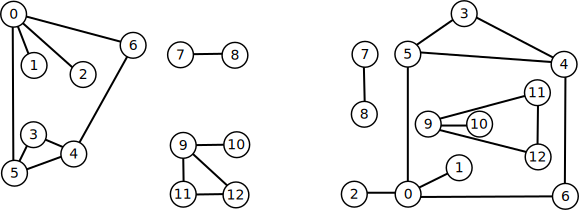
\includegraphics[scale=0.4]{{./figures/graph1}.png}
\end{center}

\item we use the names 0 through $V-1$ for the vertices in a $V$-vertex graph

\item we use the notation $v$-$w$ to refer to an edge that connects vertices $v$ and $w$

\item a self-loop is an edge that connects a vertex to itself

\item parallel edges are edges that connect the same pair of vertices  
\end{itemize}
\end{frame}

\begin{frame}[fragile]
\begin{minipage}{220pt}
\begin{itemize}
\item the degree of a vertex is the number of vertices connected to it

\item  a path is a sequence of vertices connected by edges

\item a cycle is a path with at least one edge whose first and last vertices are the same

\item the length of a path or a cycle is its number of edges

\item a graph is connected if there is a path from every vertex to every other vertex in the graph

\item a graph that is not connected consists of a set of connected components, which are maximal connected subgraphs

\item an acyclic graph is a graph with no cycles

\item a tree is an acyclic connected graph

\item a bipartite graph is a graph whose vertices can be divided into two sets such that all edges connect a vertex in one set with a vertex in the other set
\end{itemize}
\end{minipage}%
\begin{minipage}{100pt}
\begin{center}
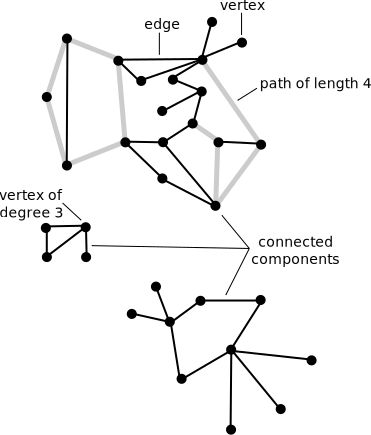
\includegraphics[scale=0.45]{{./figures/graph2}.png}

\tiny anatomy of a graph

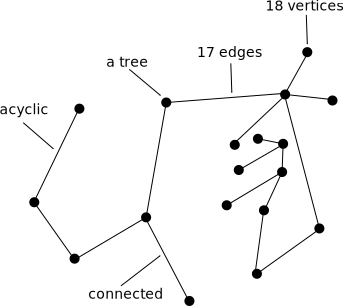
\includegraphics[scale=0.45]{{./figures/graph3}.png}

\tiny a tree

\includegraphics[scale=0.45]{{./figures/bipartite}.png}

\tiny a bipartite graph
\end{center}
\end{minipage}
\end{frame}

\begin{frame}[fragile]
\begin{itemize}
\item graph applications
\begin{center}
\begin{tabular}{ccc}
\textbf{graph} & \textbf{vertex} & \textbf{edge} \\ \hline \\
communication & telephone, computer & fiber optic cable \\
circuit & gate, register, processor & wire \\
mechanical & joint & rod, beam, spring \\
financial & stock, currency & transactions \\
transportation & intersection & street \\
internet & class C network & connection \\
game & board position & legal move \\
social relationship & person & friendship \\
neural network & neuron & synapse \\
protein network & protein & protein-protein interaction \\
molecule & atom & bond
\end{tabular}  
\end{center}
\end{itemize}
\end{frame}

\begin{frame}[fragile]
\begin{itemize}
\item Internet

\smallskip

\begin{center}
\includegraphics[scale=0.1]{{./figures/internet}.png}
\end{center}
\end{itemize}
\end{frame}

\begin{frame}[fragile]
\begin{itemize}
\item facebook

\smallskip

\begin{center}
\includegraphics[scale=0.25]{{./figures/facebook}.png}
\end{center}
\end{itemize}
\end{frame}

\begin{frame}[fragile]
\begin{itemize}
\item c.elegans connectome

\smallskip

\begin{center}
\includegraphics[scale=0.12]{{./figures/celegans}.png}
\end{center}
\end{itemize}
\end{frame}

\begin{frame}[fragile]
\begin{itemize}
\item coauthorship

\smallskip

\begin{center}
\includegraphics[scale=0.25]{{./figures/erdos}.png}
\end{center}
\end{itemize}
\end{frame}

\begin{frame}[fragile]
\begin{itemize}
\item some graph-processing problems
\begin{center}
\begin{tabular}{cc}
\textbf{problem} & \textbf{description} \\ \hline \\
$s$-$t$ path & is there a path between $s$ and $t$? \\ 
shortest $s$-$t$ path & what is the shortest path between $s$ and $t$? \\
cycle & is there a cycle in the graph? \\
Euler cycle & is there a cycle that uses each edge exactly once? \\
Hamilton cycle & is there a cycle that uses each vertex exactly once? \\
connectivity & is there a way to connect all of the vertices? \\
biconnectivity & is there a vertex whose removal disconnects the graph? \\
bipartiteness & is a graph bipartite? \\ 
planarity & can the graph be drawn in the plane with no crossing edges? \\
graph isomorphism & do two graph representations denote the same graph?
\end{tabular}  
\end{center}
\end{itemize}
\end{frame}

\section{Undirected Graphs}
\begin{frame}[fragile]
\begin{itemize}
\item undirected graph API
\begin{lstlisting}[language={},mathescape]
public class Graph

    Graph(int V) // create a $V$-vertex graph with no edges
    Graph(In in) // read a graph from input stream in
    int V()      // number of vertices
    int E()      // number of edges
    void addEdge(int v, int w)   // add edge $v$-$w$ to this graph
    Iterable<Integer> adj(int v) // vertices adjacent to $v$
\end{lstlisting}

\item graph input format
\begin{minipage}{150pt}
\begin{lstlisting}[language={}]
$ more tinyG.txt
13 13
0 5
4 3
0 1
9 12
6 4
5 4
0 2
11 12
9 10
0 6
7 8
9 11
5 3
\end{lstlisting}
\end{minipage}%
\begin{minipage}{150pt}
\begin{center}
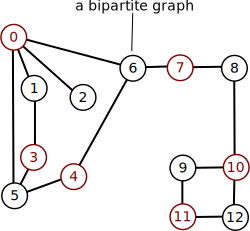
\includegraphics[scale=0.5]{{./figures/graph4}.png}
\end{center}
\end{minipage}

\item typical graph-processing code
\begin{lstlisting}[language=Java]
public static int degree(Graph G, int v) {
    int degree = 0;
    for (int w : G.adj(v)) { degree++; }
    return degree;
}
\end{lstlisting}
\end{itemize}
\end{frame}

\begin{frame}[fragile]
\begin{itemize}
\item graph representations
\begin{itemize}
\item edge list: maintain a list of the edges (linked list or array)

\item adjacency matrix: maintain a $V$-by-$V$ matrix $M$, such that $M[v][w]$ is 1 if there is an edge from $v$ to $w$, and 0 otherwise

\item adjacency list: maintain a vertex-indexed array of lists
\end{itemize}

\begin{center}
\begin{tabular}{ccccc}
\textbf{representation} & \textbf{space} & \textbf{add edge} & \textbf{is $v$-$w$ an edge?} & \textbf{enumerate \lstinline{adj(v)}} \\ \hline \\
edge list & $E$ & 1 & $E$ & $E$ \\
adjacency matrix & $V^2$ & 1$^\dagger$ & 1 & $V$ \\ 
adjacency list & $E+V$ & 1 & $degree(v)$ & $degree(v)$ 
\end{tabular}  

\smallskip

\small $\dagger$ disallows parallel edges
\end{center}
\end{itemize}
\end{frame}

\begin{frame}[fragile]
\begin{itemize}
\item implementation
\begin{lstlisting}[language=Java]
public class Graph {
    private final int V;
    private int E;
    private LinkedBag<Integer>[] adj;

    public Graph(int V) {
        if (V < 0) {
            throw new IllegalArgumentException(...); 
        }
        this.V = V;
        this.E = 0;
        adj = (LinkedBag<Integer>[]) new LinkedBag[V];
        for (int v = 0; v < V; v++) {
            adj[v] = new LinkedBag<Integer>();
        }
    }

    public Graph(In in) {
        this(in.readInt());
        int E = in.readInt();
        if (E < 0) { 
            throw new IllegalArgumentException(...);
        }
        for (int i = 0; i < E; i++) {
            int v = in.readInt();
            int w = in.readInt();
            addEdge(v, w);
        }
    }
    ...
}
\end{lstlisting}
\end{itemize}
\end{frame}

\begin{frame}[fragile]
\begin{itemize}
\item implementation (contd.)
\begin{lstlisting}[language=Java]
public class Graph {
    ...
    public int V() { return V; }

    public int E() { return E; }
 
    private void validateVertex(int v) {
        if (v < 0 || v >= V) {
            throw new IndexOutOfBoundsException(...);
        }
    }

    public void addEdge(int v, int w) {
        validateVertex(v);
        validateVertex(w);
        E++;
        adj[v].add(w);
        adj[w].add(v);
    }

    public Iterable<Integer> adj(int v) {
        validateVertex(v);
        return adj[v];
    }
    ...
}
\end{lstlisting}
\end{itemize}
\end{frame}

\section{Depth-First Search (DFS)}
\begin{frame}[fragile]
\begin{minipage}{210pt}
\begin{itemize}
\item goal: systematically traverse a graph

\item idea: mimic maze exploration

\item typical applications
\begin{itemize}
\item find all vertices connected to a given source vertex

\item find a path between two vertices
\end{itemize}

\item to visit a vertex $v$
\begin{itemize}
\item mark vertex $v$ as visited

\item recursively visit all unmarked vertices adjacent to $v$
\end{itemize}

\item data structures
\begin{itemize}
\item Boolean array \lstinline{marked[][]} to mark visited vertices

\item integer array \lstinline{edgeTo[]} to keep track of paths; \lstinline{edgeTo[w] = v} means that edge $v$-$w$ taken to visit $w$ for first time

\item function-call stack for recursion
\end{itemize}
\end{itemize}
\end{minipage}
\begin{minipage}{90pt}
\begin{center}
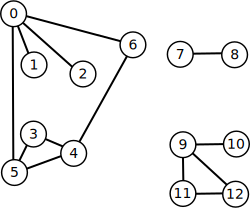
\includegraphics[scale=0.4]{{./figures/graph5}.png}

\smallskip

\small depth-first maze exploration
\end{center}
\end{minipage}
\end{frame}

\begin{frame}[fragile]
\begin{itemize}
\item design pattern for graph processing: decouple graph data type from graph processing
\begin{itemize}
\item create a \lstinline{Graph} object

\item pass the \lstinline{Graph} object to a graph-processing routine

\item query the graph-processing routine for information
\end{itemize}

\begin{lstlisting}[language={},mathescape]
public class Paths

    Paths(Graph G, int s)           // find paths in $G$ from source $s$
    boolean hasPathTo(int v)        // is there a path from $s$ to $v$?
    Iterable<Integer> pathTo(int v) // path from $s$ to $v$, or null
\end{lstlisting}

\begin{lstlisting}[language=Java]
    ...
    Paths paths = new Paths(G, s);
    for (int v = 0; v < G.V(); v++) {
        if (paths.hasPathTo(v)) {
            StdOut.println(v);
        }
    }
    ...
\end{lstlisting}
\end{itemize}
\end{frame}

\begin{frame}[fragile]
\begin{itemize}
\item depth-first search: implementation
\begin{lstlisting}[language=Java]
public class DepthFirstPaths {
    private boolean[] marked; 
    private int[] edgeTo; 
    private final int s; 

    public DepthFirstPaths(Graph G, int s) {
        this.s = s;
        edgeTo = new int[G.V()];
        marked = new boolean[G.V()];
        dfs(G, s);
    }

    private void dfs(Graph G, int v) {
        marked[v] = true;
        for (int w : G.adj(v)) {
            if (!marked[w]) {
                edgeTo[w] = v;
                dfs(G, w);
            }
        }
    }

    public boolean hasPathTo(int v) { return marked[v]; }

    public Iterable<Integer> pathTo(int v) {
        if (!hasPathTo(v)) { return null; }
        LinkedStack<Integer> path = new LinkedStack<Integer>();
        for (int x = v; x != s; x = edgeTo[x]) { path.push(x); }
        path.push(s);
        return path;
    }
    ...
}
\end{lstlisting}
\end{itemize}
\end{frame}

\begin{frame}[fragile]
\begin{itemize}
\item depth-first search: trace
\begin{center}
\includegraphics[scale=0.37]{{./figures/graph6}.png}

\smallskip

\small trace of depth-first search to find vertices connected to 0
\end{center}
\end{itemize}
\end{frame}

\section{Breadth-First Search (BFS)}
\begin{frame}[fragile]
\begin{minipage}{210pt}
\begin{itemize}
\item goal: given a graph and a source vertex $s$, support queries of the form
\begin{itemize}
\item is there a path from $s$ to a given target vertex $v$?

\item if so, find a shortest such path (one with minimal number of edges)
\end{itemize}

\item repeat until queue is empty
\begin{itemize}
\item remove vertex $v$ from queue

\item add to queue all unmarked vertices adjacent to v and mark them
\end{itemize}
\end{itemize}
\end{minipage}
\begin{minipage}{90pt}
\begin{center}
\includegraphics[scale=0.4]{{./figures/graph7}.png}

\smallskip

\small breadth-first maze exploration
\end{center}
\end{minipage}
\end{frame}

\begin{frame}[fragile]
\begin{itemize}
\item breadth-first search: implementation
\begin{lstlisting}[language=Java]
public class BreadthFirstPaths {
    private static final int INFINITY = Integer.MAX_VALUE;
    private boolean[] marked; 
    private int[] edgeTo; 
    private int[] distTo;   

    public BreadthFirstPaths(Graph G, int s) {
        marked = new boolean[G.V()];
        distTo = new int[G.V()];
        edgeTo = new int[G.V()];
        bfs(G, s);
    }

    private void bfs(Graph G, int s) {
        LinkedQueue<Integer> q = new LinkedQueue<Integer>();
        for (int v = 0; v < G.V(); v++) { distTo[v] = INFINITY; }
        distTo[s] = 0;
        marked[s] = true;
        q.enqueue(s);
        while (!q.isEmpty()) {
            int v = q.dequeue();
            for (int w : G.adj(v)) {
                if (!marked[w]) {
                    edgeTo[w] = v;
                    distTo[w] = distTo[v] + 1;
                    marked[w] = true;
                    q.enqueue(w);
                }
            }
        }
    }
    ...
}
\end{lstlisting}
\end{itemize}
\end{frame}

\begin{frame}[fragile]
\begin{itemize}
\item breadth-first search: implementation (contd.)
\begin{lstlisting}[language=Java]
public class BreadthFirstPaths {
    ...
    public boolean hasPathTo(int v) { return marked[v]; }

    public int distTo(int v) { return distTo[v]; }

    public Iterable<Integer> pathTo(int v) {
        if (!hasPathTo(v)) return null;
        LinkedStack<Integer> path = new LinkedStack<Integer>();
        int x;
        for (x = v; distTo[x] != 0; x = edgeTo[x]) {
            path.push(x);
        }
        path.push(x);
        return path;
    }
    ...
}
\end{lstlisting}
\end{itemize}
\end{frame}

\begin{frame}[fragile]
\begin{itemize}
\item breadth-first search: trace
\begin{center}
\includegraphics[scale=0.37]{{./figures/graph8}.png}

\smallskip

\small trace of breadth-first search to find all paths from 0
\end{center}
\end{itemize}
\end{frame}

\section{Connected Components}
\begin{frame}[fragile]
\begin{itemize}
\item vertices $v$ and $w$ are connected if there is a path between them

\item goal: preprocess graph to answer queries of the form \emph{is $v$ connected to $w$} in constant time

\begin{lstlisting}[language={},mathescape]
public class CC

    CC(Graph G)                     // find connected components in $G$
    boolean connected(int v, int w) // are $v$ and $w$ connected?
    int count()     // number of connected components
    int id(int v)   // component identifier for $v$ from $[0, \text{count()} - 1]$
    int size(int v) // number of vertices in $v$'s component
\end{lstlisting} 

\smallskip

use union-find? not quite

\smallskip

use depth-first search? yes
\end{itemize}
\end{frame}

\begin{frame}[fragile]
\begin{itemize}
\item connected components: implementation
\begin{lstlisting}[language=Java]
public class CC {
    private boolean[] marked; 
    private int[] id; 
    private int[] size;  
    private int count;  
    
   public CC(Graph G) {
        marked = new boolean[G.V()];
        id = new int[G.V()];
        size = new int[G.V()];
        for (int v = 0; v < G.V(); v++) {
            if (!marked[v]) {
                dfs(G, v);
                count++;
            }
        }
    }

    private void dfs(Graph G, int v) {
        marked[v] = true;
        id[v] = count;
        size[count]++;
        for (int w : G.adj(v)) { if (!marked[w]) { dfs(G, w); } }
    }
    
    public boolean connected(int v, int w) { return id(v) == id(w); }

    public int count() { return count; }

    public int id(int v) { return id[v]; }

    public int size(int v) { return size[id[v]]; }
    ...
}
\end{lstlisting} 
\end{itemize}
\end{frame}

\section{Graph Traversal Summary}
\begin{frame}[fragile]
\begin{itemize}
\item BFS and DFS enables efficient solution of many (but not all) graph problems
\begin{center}
\begin{tabular}{cccc}
\textbf{problem} & \textbf{BFS} & \textbf{DFS} & \textbf{time} \\ \hline \\
path between $s$ and $t$ & \cmark & \cmark & $E + V$ \\
shortest path between $s$ and $t$ & \cmark & & $E+V$ \\
cycle & \cmark & \cmark & $E+V$ \\
Euler cycle & & \cmark & $E+V$ \\
Hamilton cycle & & & $2^{1.657V}$ \\
connected components & \cmark & \cmark & $E+V$ \\
biconnected components & & \cmark & $E+V$ \\
bipartiteness & \cmark & \cmark & $E+V$ \\
planarity & & \cmark & $E+V$ \\
graph isomorphism & & & $2^{c\sqrt{V\log V}}$ 
\end{tabular} 
\end{center}
\end{itemize}
\end{frame}

\end{document}
